\documentclass{article}

\usepackage[french]{babel}
\usepackage[T1]{fontenc}
\usepackage{moreverb}       % verbatim with tab

\usepackage{wrapfig}
\usepackage{graphicx}
\usepackage{geometry}
\geometry{hmargin=2.5cm}
\usepackage{amsmath}
\usepackage{siunitx}

\usepackage{graphicx}
\usepackage{subcaption}
\usepackage{float}
\usepackage{hyperref}
\usepackage{setspace}
\usepackage{xcolor}
\usepackage{pdfpages}
\usepackage{enumitem}
\usepackage{lscape}

\usepackage{fancyhdr}       % en-têtes
\usepackage{lastpage}       % numéro de dernière page

\title{Systèmes logiques programmés\bigbreak \bigbreak
    \large Dossier récapitulatif\bigbreak
    \normalsize Programmation d'un générateur de signaux en assembleur sur PIC16F887\bigbreak}
\date{2020 -- 2021}
\author{Laura Binacchi}

\pagestyle{fancy}
\renewcommand\headrulewidth{1pt}
\fancyhead[L]{Laura Binacchi}
\fancyhead[C]{Systèmes logiques programmés}
\fancyhead[R]{\today}


\begin{document}
    \pagenumbering{gobble}
    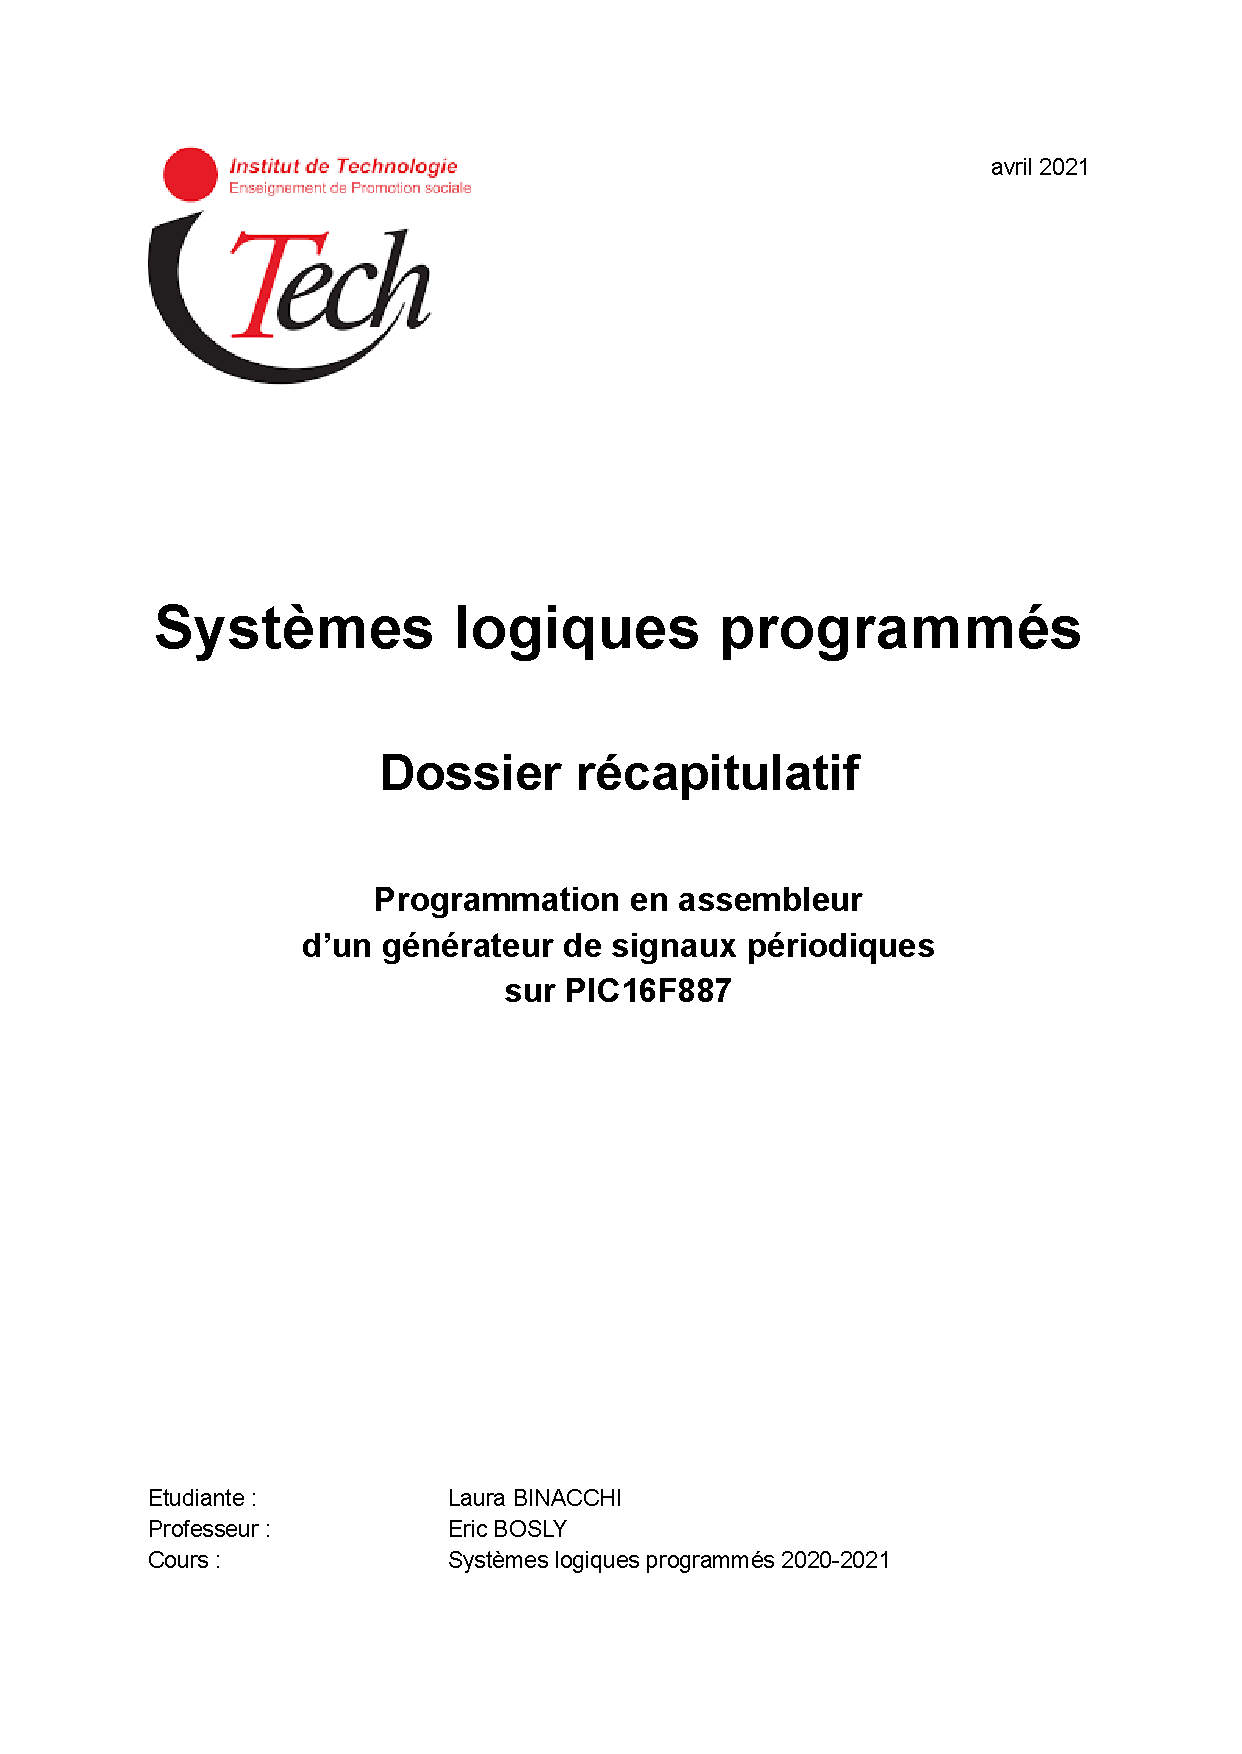
\includepdf[pages={1}]{pdg}
    \newpage
    \tableofcontents
    \newpage
    \pagenumbering{arabic}

    \section{Cahier des charges}
    \paragraph{}
    Sur base des modules élémentaires et exemples vus au cours (ports, interruptions, timers, CCP, SPI, I2C, ADC, LCD) développer sous MPLABX une application en langage d’assemblage sur PIC série 16F8xx ou 16F9xx ainsi que le modèle Proteus permettant de la simuler. L’application devra utiliser au moins une source d’interruptions, gérer un LCD et connecter au moins un circuit esclave en mode SPI ou I2C.

    \paragraph{}
    L’application permettra de générer un signal simple, carré ou triangulaire, de fréquence et rapport cyclique paramétrables. Le signal sera généré par l’intermédiaire d’un DAC 8 bits.

    \paragraph{}
    Les datasheets des PIC et des circuits nécessaires sont données, vous pouvez en choisir d’autres si vous le souhaitez et que cela se justifie. Vous ne devez évidemment pas utiliser tous les circuits, juste ceux nécessaires pour votre application. Une routine de conversion binaire / BCD est également donnée.

    \paragraph{}
    Les caractéristiques de l'applications sont données dans la liste ci-dessous. Vous avez le choix du dispositif de saisie (boutons, clavier, roue codeuse, dip switch, ...) et de la taille de l’écran, minimum 2x16 caractères. Vous pouvez faire plus que demandé, pas moins.
    \begin{itemize}[label=$\bullet$]
        \item Application : générateur de signaux
        \item PIC : 16F876A, 16F877A ou 16F887
        \item Bus : I2C
        \item Sortie signal : DAC 0808 connexion directe au PIC
        \item Paramètres : fréquence, type et rapport cyclique du signal
        \item LCD : connexion au bus I2C via IO expander 16 bits
    \end{itemize}



    \section{Analyse}
    \paragraph{}
    Le générateur de signaux est implémenté par le module de comparaison du microcontrôleur : une interruption est générée à un intervalle régulier pour mettre à jour la valeur du signal sur le convertisseur numérique analogique.

    \paragraph{}
    Les valeurs du signal sont stockées dans un vecteur de 100 bytes initialisé au démarrage de la génération de signal. A chaque itération de l'interruption déclenchée par le module CCP, la valeur du signal est récupérée et projetée sur le DAC. La gamme de PIC proposée ne disposant pas de banque assez grande pour stocker un vecteur de cette taille, le tableau de 100 valeurs représentant le signal est stocké dans deux vecteurs de 50 bytes répartis sur les banques 2 et 3.

    \paragraph{}
    Le signal généré doit être paramétrable : il faut donc implémenter un mode de configuration. Celui-ci est totalement indépendant du mode de génération du signal : les deux modes de fonctionnement ne peuvent pas être concurrents car ils utilisent tous deux des interruptions et que la gamme de microcontrôleurs PIC16F ne permet pas de donner un niveau de priorité supérieur à une interruption sur l'autre. Les deux interruptions ne sont donc pas activées en même temps : le mode de génération du signal active l'interruption par le module CCP et désactive l'interruption sur la PIN RB0 et le mode de configuration fait l'inverse.

    \paragraph{}
    Un switch permet de choisir le mode de fonctionnement. Il est testé en polling par la boucle principale du programme. Avec un PIC qui supporte l'implémentation de niveaux de priorité les deux interruptions pourront être activées en même temps avec une priorité donnée à l'interruption qui génère le signal. Le programme n'aurait alors plus besoin d'implémenter deux modes de fonctionnement et de tester en boucle la valeur du switch.

    \paragraph{}
    Une LED permet de le visualiser le mode de fonctionnement : elle est allumée lorsque le signal est généré et éteinte en mode de configuration.

    \paragraph{}
    Un écran LCD permet de visualiser les paramètres du signal : forme du signal, fréquence, rapport cyclique et amplitude. Le microcontrôleur communique avec le LCD via son bus I$^2$C par l'intermédiaire d'un I/O expander 16 bits (ce qui permet de configurer le LCD en mode 8 bits).

    \paragraph{}
    Un ensemble de sept boutons permet de régler les paramètres du signal. Cet ensemble de boutons est lui aussi connecté au microcontrôleur via son bus I$^2$C et un I/O expander de 8 bits. L'I/O expander génère une interruption sur la PIN RB0 du microcontrôleur lorsqu'une entrée est détectée.

    \paragraph{}
    La sélection de la forme du signal se fait par un seul bouton qui permet de faire défiler la forme du signal : initialisé à carré, il passe ensuite à triangulaire, puis dent de scie, puis carré et ainsi de suite. Le signal en dent de scie est une forme particulière du signal triangulaire dont le rapport cyclique est égal à 0 ou à 100\%. Il aurait pu ne pas être répété : l'implémenter permet toutefois de sélectionner plus rapidement cette forme de signal plutôt qu'en paramétrant le rapport cyclique du signal triangulaire.

    \paragraph{}
    La fréquence peut être augmentée et diminuée par deux boutons différents. Elle est initialisée à \SI{1}{\kilo\hertz} et peut-être diminuée en augmentant la valeur du prescaler du timer qui génère l'interruption : elle sera donc divisée par deux pour atteindre une valeur minimum de \SI{125}{\hertz} (prescaler 1:8). La fréquence aurait également pu être diminuée en augmentant la valeur de comparaison du module CCP : le pas de diminution aurait alors pu être plus fin. La fréquence aurait également pu être réglée en diminuant le nombre de valeurs du tableau affichées : elle aurait été doublée en n'affichant qu'une valeur sur deux, etc. Le générateur aurait alors pu monter à des fréquences plus élevées mais au prix d'un signal moins lisse.

    \paragraph{}
    La rapport cyclique est réglé par deux boutons. Il s'exprime en pourcentage et peut être diminué et augmenté par pas de 10\%. Ses valeurs sont comprises entre 0 et 100\% inclus.

    \paragraph{}
    L'amplitude du signal s'exprime elle aussi en pourcentage : il s'agit d'un pourcentage de la tension de référence donnée au convertisseur numérique-analogique. L'amplitude varie comme le rapport cyclique entre 0 et 100\% par pas de 10 et est réglée par deux boutons.

    \paragraph{}
    Les différents réglages des paramètres nécessitent l'implémentation d'une arithmétique entière non signée sur 16 bits, e.g. pour diviser la fréquence par deux. L'affichage des paramètres nécessite quant à lui l'implémentation de routines de conversion des nombres binaires vers du BCD.


    \section{Choix du matériel}
    \paragraph{}
    Le développement du générateur de signaux périodique se base sur un hardware composé de :
    \begin{itemize}[label=$\bullet$]
        \item un microcontrôleur \textbf{PIC16F887};
        \item un \textbf{switch} connecté directement au microcontrôleur (PORTC, 0) permettant de sélectionner le mode de fonctionnement : génération de signal (switch fermé) ou configuration du signal (switch ouvert);
        \item une \textbf{LED} connectée directement au microcontrôleur (PORTC, 1) pour visualiser le mode de fonctionnement;
        \item un convertisseur numérique-analogique \textbf{DAC0808} connecté directement au port D du microcontrôleur;
        \item un écran LCD \textbf{LM044L} (de $4\times 20$ caractères) connecté via un I/O expander 16 bits \textbf{PCA9535} (bus I$^2$C) pour afficher les paramètres du signal;
        \item sept boutons connectés via un I/O expander 8 bits \textbf{PCA9554} (bus I$^2$C) pour paramétrer le signal.
    \end{itemize}

    \paragraph{}
    Parmi les microcontrôleurs proposés, j'ai choisi le PIC16F887. J'ai écarté le PIC16F876A car il n'est pas recommandé par \emph{Microchip} pour les nouveaux développements\footnote{Voir la mention \emph{Status: Not Recommended for new designs} affichée sur site du fabricant \url{https://www.microchip.com/wwwproducts/en/PIC16F876A}}. Le PIC16F887 a plus de fonctionnalités que le PIC16F877A, e.g plus de PIN qui peuvent être configurées en analogique et un mode ECCP. Ces fonctionnalités ne sont pas utiles pour le générateur de signaux. J'ai tout de même choisi ce microcontrôleur car il est deux fois moins cher que le PIC16F877A\footnote{Prix de référence sur le site du fabricant : 2,60 euros pour le PIC16F887-I/P contre 4,56 euros pour le PIC16F877A-I/P et 4,39 euros pour le PIC16LF876A-I/SP.}.

    \paragraph{}
    Le DAC0808 est connecté directement au microcontrôleur et pas via bus de communication. C'est la manière la plus rapide de le connecter au microcontrôleur : la valeur est directement envoyée au DAC sans le temps supplémentaire nécessaire à l'envoi par un bus de communication (envoi des conditions de démarrage et de fin de communication, envoi de chaque bit les uns à la suite des autres, etc).

    \paragraph{}
    Le choix du mode de fonctionnement est fait par un switch plutôt que par un bouton car il n'y a que deux modes de fonctionnement : la valeur de la PIN à laquelle est connecté le switch peut donc être testée directement sans devoir garder en mémoire le mode choisi.

    \paragraph{}
    Le mode de fonctionnement est visualisé par une LED plutôt qu'affiché sur le LCD afin de ne garder le LCD que pour l'affichage des paramètres du signal.

    \paragraph{}
    J'ai choisi un LCD de 4 lignes (deux de plus que le minimum recommandé) pour pouvoir afficher un paramètre par ligne et donc privilégier la lisibilité des paramètres. Il est connecté au microcontrôleur via l'I/O expander recommandé dans les consignes pour la communication I$^2$C.

    \paragraph{}
    Les entrées sont elles aussi connectées via un I/O expander du même fabricant que l'I/O expander du LCD mais en 8 bits (suffisants pour connecter les 7 entrées). Les changements de paramètres pourront ainsi être détectés par interruption plutôt que par polling.


    %\section{Projet Proteus}
    %\paragraph{}
    %Le projet Proteus est divisé en deux feuilles : la première présente les éléments avec lesquels l'utilisateur interagit et la seconde tous les autres éléments. Cette présentation permet de ne pas alourdir la visualisation dans Proteus.

    %\paragraph{}
    %La première feuille comprend les éléments de l'interface humain-machine :
    %\begin{itemize}[label=$\bullet$]
    % \item l'écran LCD;
    %     \item la LED de visualisation du mode de fonctionnement;
    %     \item les boutons et switch représentés par des états logiques pour simplifier le schéma;
    %     \item l'oscilloscope permettant de visualiser le signal de sortie du DAC.
    % \end{itemize}

    % \begin{figure}[H]
    %     \centering
    %     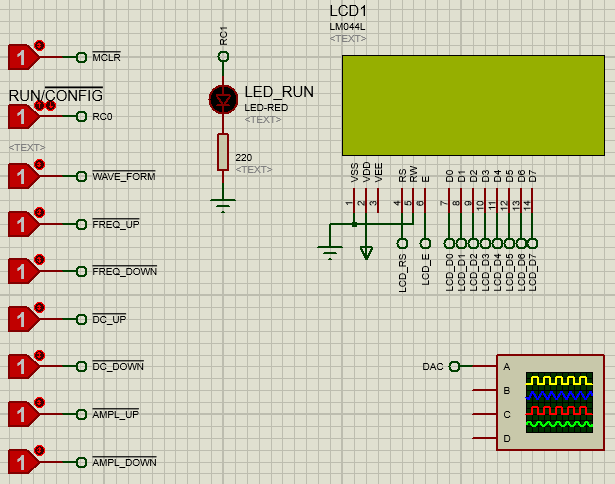
\includegraphics[width=.55\textwidth]{./images/proteus_rs1.png}
    % \end{figure}

    \newpage
    % \paragraph{}
    % La seconde feuille comprend les éléments de hardware cachés :
    % \begin{itemize}[label=$\bullet$]
    %     \item le microcontrôleur;
    %     \item les I/O expander PCA9535 et PCA9554 et les circuits associées (résistances de pull-up);
    %     \item le DAC et les circuits associés (résistances de pull-up et amplificateur opérationnel en buffer).
    % \end{itemize}

    % \begin{figure}[H]
    %     \centering
    %     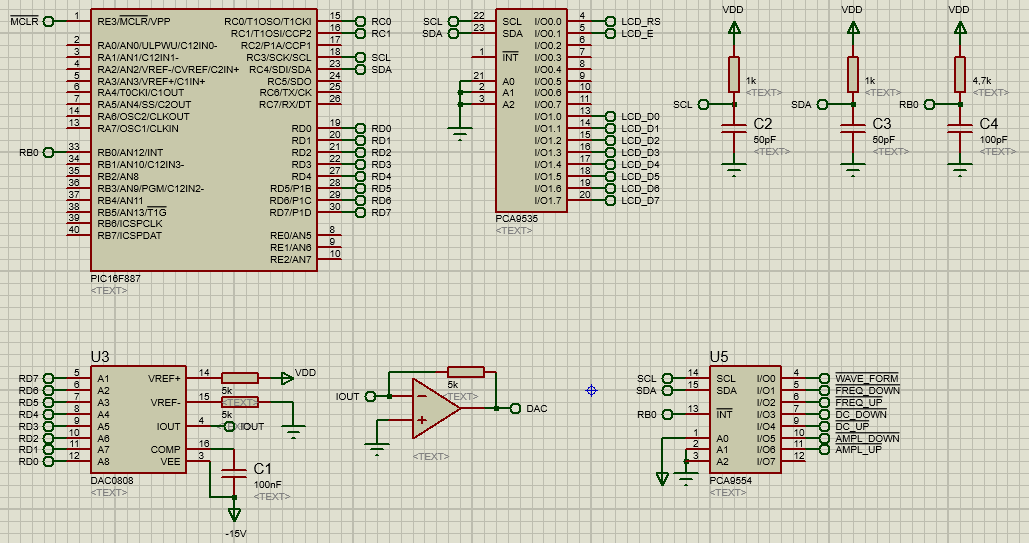
\includegraphics[width=\textwidth]{./images/proteus_rs2.png}
    % \end{figure}

    % \paragraph{}
    % Les circuits associés aux différents éléments sont ceux fournis par leurs datasheets.



    \section{Configuration}
    \paragraph{}
    Pour compiler le projet avec MPLABX, les options suivantes doivent être ajoutées au linker pour définir l'emplacement des vecteurs de reset et d'interruption : \texttt{-presetVec=0x00} et \texttt{-pinterVec=0x04}.

    \paragraph{}
    Les configurations du PIC sont définies ou appelées sous le label \texttt{init} du fichier principal à l'exception de l'activation des interruptions qui se fait à l'initialisation des modes de fonctionnement du programme (\texttt{init\_mode\_run} et \texttt{init\_mode\_config}).

    \paragraph{}
    Les ports C (LED de mode et PINs liées au bus I$^2$C) et D (DAC) sont configurés en output et mis à 0 à l'exception de la PIN RC0 à laquelle est associé le switch de sélection de mode. La PIN RB0 est configurée en input et en digital (configuration du registre \texttt{ANSELH}).

    \paragraph{}
    L'interruption sur la PIN RB0 est configurée pour être déclenchée sur un front descendant par le registre \texttt{INTEDG} car la PIN est maintenue à un état haut par le PCA9554 et passe à un état bas lorsqu'une donnée est lue. Cette interruption est activée lors du démarrage en mode de configuration ou lors du passage du mode de génération de signal au mode de configuration. Elle est désactivée lors du passage en mode de génération du signal.
 
    \paragraph{}
    L'interruption générée par le module CCP2 est configurée en mode \emph{special event trigger} : l'interruption active le flag d'interruption et réinitialise le timer associé (TIMER1). J'utilise le module CCP2 car je n'ai pas besoin des fonctionnalités supplémentaires du module ECCP1. L'interruption de ce module est activée lors du démarrage du programme en mode de génération de signal ou lors du passage du mode de configuration au mode de génération. Elle est désactivée lors du passage en mode de configuration.

    \paragraph{}
    La valeur de comparaison est initialisée à 50 (registres \texttt{CCPR2H} et \texttt{CCPR2L}). Puisque l'oscillateur du microcontrôleur est à \SI{20}{\mega\hertz}, la période d'une instruction est de \SI{0.2}{\micro\second}. Avec une valeur de comparaison à 50, une interruption sera donc déclenchée toutes les \SI{10}{\micro\second}. Cette valeur permet de vérifier facilement les fréquences du signal généré. Initialisée à 5, le temps d'exécution des instructions de l'interruption aurait dépassé le temps de l'interruption et il y aurait eu un phénomène de trashing.

    \paragraph{}
    La routine d'initialisation appelle les fonctions d'initialisation du bus I$^2$C des deux I/O expander et du LCD implémentées dans les fichiers \emph{I2C.s}, \emph{LM044L\_PCA9535.s} et \emph{PCA9554.s}. Ces routines permettent respectivement d'initialiser le bus I$^2$C à \SI{400}{\kilo\hertz} puis d'initialiser via ce bus les deux ports PCA9535 en output et le port du PCA9554 en input et enfin d'initialiser le LCD via le PCA9535.

    \paragraph{}
    Après avoir initialisé les valeurs par défauts des paramètres du signal (type carré, fréquence à \SI{1000}{\hertz}, rapport cyclique à 50\% et amplitude à 100\%), l'affichage du LCD est initialisé et les différents paramètres sont affichés. Le programme est prêt à se lancer dans le mode sélectionné.



    \newpage
    \section{Fonctionnement du programme}
    \subsection{Configuration du signal}
    \paragraph{}
    A l'initialisation du mode de configuration du signal, l'interruption du module CCP2 est désactivée. La valeur projetée sur le port D connecté au DAC est remise à 0 et la LED d'indication de mode est éteinte. Enfin l'interruption sur le port RB0 est activée. Le programme va alors attendre une interruption tout en bouclant pour tester si le mode a été changé.

    \paragraph{}
    Lorsqu'une interruption est déclenchée par RB0, la valeur du PCA9554 est lue et est testée pour déterminer quel paramètre doit être mis à jour.

    \paragraph{}
    La forme du signal est stockée dans la variable \texttt{wave\_form} dont chacun des trois premiers bits correspond à un type de signal. Ce paramètre est modifié par rotation de bit avec un retour au premier signal une fois que le bit passe dans le \texttt{CARRY}.

    \paragraph{}
    La fréquence est modifiée par modification du prescaler du timer 1 : sa valeur augmente pour diminuer la fréquence et inversement. La valeur affichée stockée dans la variable \texttt{frequency} est divisée ou multipliée par deux avec les macros définies dans le fichier \emph{16bits\_arithmetic\_macros.inc}. Les valeurs limites sont testées pour que la fréquence ne puisse pas descendre sous  \SI{125}{\hertz} (prescaler à 1:8) et ne puisse pas monter au-dessus de \SI{1000}{\hertz} (prescaler à 1:1).

    \paragraph{}
    Le rapport cyclique et l'amplitude sont modifiés par pas de 10 entre 0 et 100\% compris. La seule exception est pour le signal en dent de scie : son rapport cyclique ne peut être que de 0 (équivalent à un signal triangulaire n'ayant qu'un front descendant) ou 100 (équivalent à un signal triangulaire n'ayant qu'un front ascendant). Lors de la sélection de cette forme de signal, si le rapport cyclique est différent de 100\%, il est automatiquement passé à 100\%.


    \subsection{Génération du signal}
    \paragraph{}
    Au démarrage du programme en mode de génération de signal ou lors du passage du mode de configuration au mode de génération, l'interruption sur RB0 est désactivée. Puis le vecteur de valeurs du signal est initialisé en fonction des paramètres du signal sélectionné ou des paramètres par défaut. Enfin l'interruption du module CCP2 est activée et le programme attend que l'interruption à intervalle régulier soit générée pour projeter la valeur du signal sur le DAC tout en bouclant sur la valeur du switch de mode au cas où le système serait repassé en mode de configuration.

    \paragraph{}
    Le vecteur de valeurs du signal est initialisé par une macro. Cette macro permet de cacher l'implémentation du vecteur en deux parties sur les banques 2 et 3. Si l'indice du tableau est inférieur à 50, le valeur du signal est stockée dans la banque 2 à l'indice demandé. Sinon, elle est stockée dans la banque 3 à l'indice - 50.

    \paragraph{}
    Puisque le signal est défini par 100 valeurs et que la durée d'une interruption est de \SI{10}{\micro\second}, la fréquence maximale du signal généré sera de $\frac{1}{100 \times 10^{-5}} = \SI{1}{\kilo\hertz}$.

    \paragraph{}
    Implémenter un vecteur de 100 valeurs pour représenter le signal permet de générer un signal assez lisse. Cela permet également de simplifier certains calculs comme le rapport cyclique sans avoir à faire de règle de trois pour adapter le pourcentage paramétré. Sur un tableau de 100 valeurs, le rapport cyclique implémenté pourrait être paramétré avec une précision de 1\% mais le programme implémente une configuration par pas de 10\% pour plus de facilité d'utilisation de l'interface.

    \paragraph{}
    Les signaux carrés sont implémentés en initialisant les \texttt{x} premières valeurs du tableau à la valeur numérique maximale du signal, \texttt{x} étant la valeur du rapport cyclique puisque celui-ci est compris entre 1 et 100, que le vecteur de valeurs a une taille de 100 bytes et que la valeur numérique du signal est codées sur un byte. La valeur du signal est calculée à partir de l'amplitude : $signal = \frac{255 \times amplitude}{100}$. Le reste du vecteur est initialisé à \texttt{0}.

    \paragraph{}
    Pour les signaux triangulaires, la valeur du signal est recalculée pour chaque emplacement du vecteur à partir de la valeur maximale du signal calculée au préalable de la même manière que pour les signaux carrés.

    \paragraph{}
    Pour le front montant, la valeur du signal évolue de 0 à la valeur maximale du signale : $signal = \frac{max \times i}{samples}$ pour \emph{i} variant de 0 au nombre d'échantillons du front montant (égal à la valeur du rapport cyclique) et \emph{samples} étant égal à la valeur du rapport cyclique.

    \paragraph{}
    Pour le front descendant, la valeur évolue de la valeur maximale du signal à 0 suivant l'équation : $signal = \frac{max \times (samples - i)}{samples}$ pour \emph{i} variant de 0 au nombre d'échantillons du front descendant (égal à 100 moins la valeur du rapport cyclique) et \emph{samples} étant égal à 100 moins la valeur du rapport cyclique.

    \paragraph{}
    Les signaux en dent de scie sont des cas particuliers de signaux triangulaires dont le rapport cyclique est de 0 ou de 100.

    \paragraph{}
    Après son initialisation, le double vecteur de valeurs du signal est exploité par une macro de récupération de la valeur implémentant le même mécanisme que la macro d'initialisation.



    % \subsection{Conversions en caractères ASCII}
    % \paragraph{}
    % Les conversions des nombres en caractères ASCII sont définies dans le fichier \emph{16bits\_bin\_bcd\_ascii.inc} et implémentées dans le fichier \emph{16bits\_bin\_bcd\_ascii.s}. Elles permettent de convertir un nombre binaire en caractères ASCII ou de le transformer en BCD pour permettre un affichage en décimal. L'affichage décimal peut se faire pour un nombre de 8 ou de 16 bits et peut donc afficher une valeurs jusqu'à 65535 (\texttt{0xFFFF}).

    % \subsection{Arithmétique 16 bits}
    % \paragraph{}
    % J'ai repris les opérations d'arithmétique 16 bits vues au cours et la séparation des fichiers contenant les macros (\emph{16\_bits\_arithmetic\_macros.inc}), les définitions des fonctions (\emph{16\_bits\_arithmetic.inc}) et l'implémentation des fonctions (\emph{16\_bits\_arithmetic.s}).

    % \paragraph{}
    % J'ai ajouté la fonction \texttt{MUL8} qui permet de multiplier deux nombres de 8 bits et d'obtenir un résultats de 16 bits. J'ai également ajouté le test de la valeur \texttt{0} pour le dividende de la division 16 bits.

    % \paragraph{}
    % Toutes les macros et fonctions ne sont pas utilisées mais elles sont laissées dans les fichiers pour pouvoir réutiliser ceux-ci dans d'autres projets.



    \section{Tests}
    \paragraph{}
    J'ai testé le paramétrage du signal dans Proteus en faisant passer les paramètres par toutes les valeurs possibles et en vérifiant que les affichages correspondent bien aux changements attendus. Ce test m'a permis de vérifier que le programme ne permette pas de dépasser les valeurs limites des paramètres : 0 et 100 pour le rapport cyclique et l'amplitude et 125 et 1000 pour la fréquence.

    \paragraph{}
    L'adéquation entre les paramètres du signal et le signal produit est vérifiée par l'observation du signal à l'oscilloscope : elle permet de vérifier la forme du signal, sa fréquence, son rapport cyclique et son amplitude assez facilement avec les paramètres possibles du signal.

    \paragraph{}
    Tout au long du développement, j'ai vérifié les valeurs contenues dans les différents registres du PIC grâce à l'outil \emph{Watch Window} des options de debug de Proteus. J'ai également vérifié régulièrement les valeurs des PIN en les connectant à l'oscilloscope. Par exemple, pour mettre en place la communication du LCD via le bus I$^2$C, j'ai vérifié la valeur contenue dans le registre \texttt{SSPBUF} et j'ai vérifié les états des PIN SDA et SCL à l'oscilloscope.

    \paragraph{}
    A partir du moment où mon programme implémentait le LCD et où il est devenu trop complexe que pour retrouver facilement l'adresse d'une variable, j'ai utilisé le LCD et la conversion binaire vers ASCII pour vérifier les différentes valeurs intermédiaires des calculs de paramètres.



    \section{Problèmes rencontrés}
    \paragraph{}
    J'ai principalement rencontré des problèmes au début du projet pour la configuration du PIC et pour aller chercher les bonnes informations aux bons endroits dans la datasheet. Par exemple, pour la configuration de l'interruption sur RB0, le registre ANSELH devait être configuré pour que la PIN soit en mode digital et pas analogique comme elle l'est par défaut et cette information ne se trouve pas dans la section portant sur l'interruption par RB0 mais dans celle portant sur la configuration du PORTB. A force de me référer aux datasheets, leur lecture est devenue de plus en plus facile.

    \paragraph{}
    La mise en place du LCD a également été compliquée car je n'ai pas procédé par étapes mais j'ai voulu tout mettre en place d'un coup : le LCD, l'I/O expander et la communication I$^2$C. Il a alors été plus compliqué de trouver la source des erreurs de configuration et si ces erreurs étaient dues à des erreurs de configuration matérielle ou à des erreurs de programmation. Cette difficulté a été surmontée par l'utilisation des outils de debug de Proteus que j'ai ensuite utilisés pour le développement du reste du projet. Par la suite, j'ai également procédé de manière plus progressive en validant les plus petites étapes possibles à la fois et ne pas perdre du temps à chercher la source des erreurs.

    \paragraph{}
    Enfin j'ai parfois fait des choix de programmation ou des choix de matériel qui n'étaient pas en adéquation avec les possibilités du système. J'ai par exemple voulu connecter un clavier au microcontrôleur via un bus I$^2$C avant de me rendre compte de difficultés que je n'avais pas anticipées. L'expérience acquise de ces erreurs m'a permis d'acquérir une meilleure capacité d'analyse pour la réalisation de projets futurs.
\end{document}